%% Простая презентация с примером включения программного кода и
%% пошаговых спецэффектов
\documentclass{beamer}
\usepackage{fontspec}
\usepackage{xunicode}
\usepackage{xltxtra}
\usepackage{xecyr}
\usepackage{hyperref}
\setmainfont[Mapping=tex-text]{DejaVu Serif}
\setsansfont[Mapping=tex-text]{DejaVu Sans}
\setmonofont[Mapping=tex-text]{DejaVu Sans Mono}
\usepackage{polyglossia}
\setdefaultlanguage{russian}
\usepackage{graphicx}
\usepackage{listings}
\lstdefinestyle{mycode}{
  belowcaptionskip=1\baselineskip,
  breaklines=true,
  xleftmargin=\parindent,
  showstringspaces=false,
  basicstyle=\footnotesize\ttfamily,
  keywordstyle=\bfseries,
  commentstyle=\itshape\color{gray!40!black},
  stringstyle=\color{red},
  numbers=left,
  numbersep=5pt,
  numberstyle=\tiny\color{gray},
}
\lstset{escapechar=@,style=mycode}






% счетчик слайдов
\addtobeamertemplate{navigation symbols}{}{%
    \usebeamerfont{footline}%
    \usebeamercolor[fg]{footline}%
    \hspace{1em}%
    \insertframenumber/\inserttotalframenumber
}
\usepackage{graphicx}       % работа с картинками
\usepackage[export]{adjustbox}  % еще про место картинки (width,right/left])
\usepackage{multicol,caption,float, subfig} % картинки

\usepackage{multirow} % для няшных табличек      

\usepackage{hyperref} 



\begin{document}
\title{Методы машинного обучения \\в задаче предсказания погоды}
\subtitle{предварительные результаты}
\author{Лена Волжина\\{\footnotesize\textcolor{gray}{руководитель Е.Г. Михайлова}}}
\institute{СПбГУ, мат-мех, кафедра ИАС}
\date{27 декабря 2017г}
\frame{\titlepage}

\begin{frame}\frametitle{Введение}
\begin{itemize}
    % что мы называем погодой?
    \item Погода -- состояние нижнего слоя атмосферы % (нижней тропосферы) в определённом месте в определённое время
    
    % что её характеризует?
    \item Температура, погодное явление, влажность, давление, ветер, ...
    
    % как мы можем её измерить?
    \item Метеостанции, радиозонды, спутники
    
    % как делается прогноз?
    \item Численный прогноз погоды % Газодинамика, ур-ния Навье-Стокса описывают движение вязкой жидкости, не решены аналитически
    
    % это сложно, всего порядка 10 независимых организаций
    \item Глобальные модели: GFS, JMA, ECMWF, CMC; региональная: WRF
    
    % модели устаревают, обновлять их дико дорого, ошибки могут иметь тренды, машинное обучение!
    \item Машинное обучение: The Weather Company~(IBM), Яндекс.Погода
    
    %\item<2-> {\Large \textcolor{blue}{}}
\end{itemize}
\end{frame}


% Я использовала матрикснет, он работает как градиентный бустинг над решающими деревьями

\begin{frame}\frametitle{Решающие деревья}
    \begin{figure}[t]
      \centering
      \subfloat[классификация наблюдений]{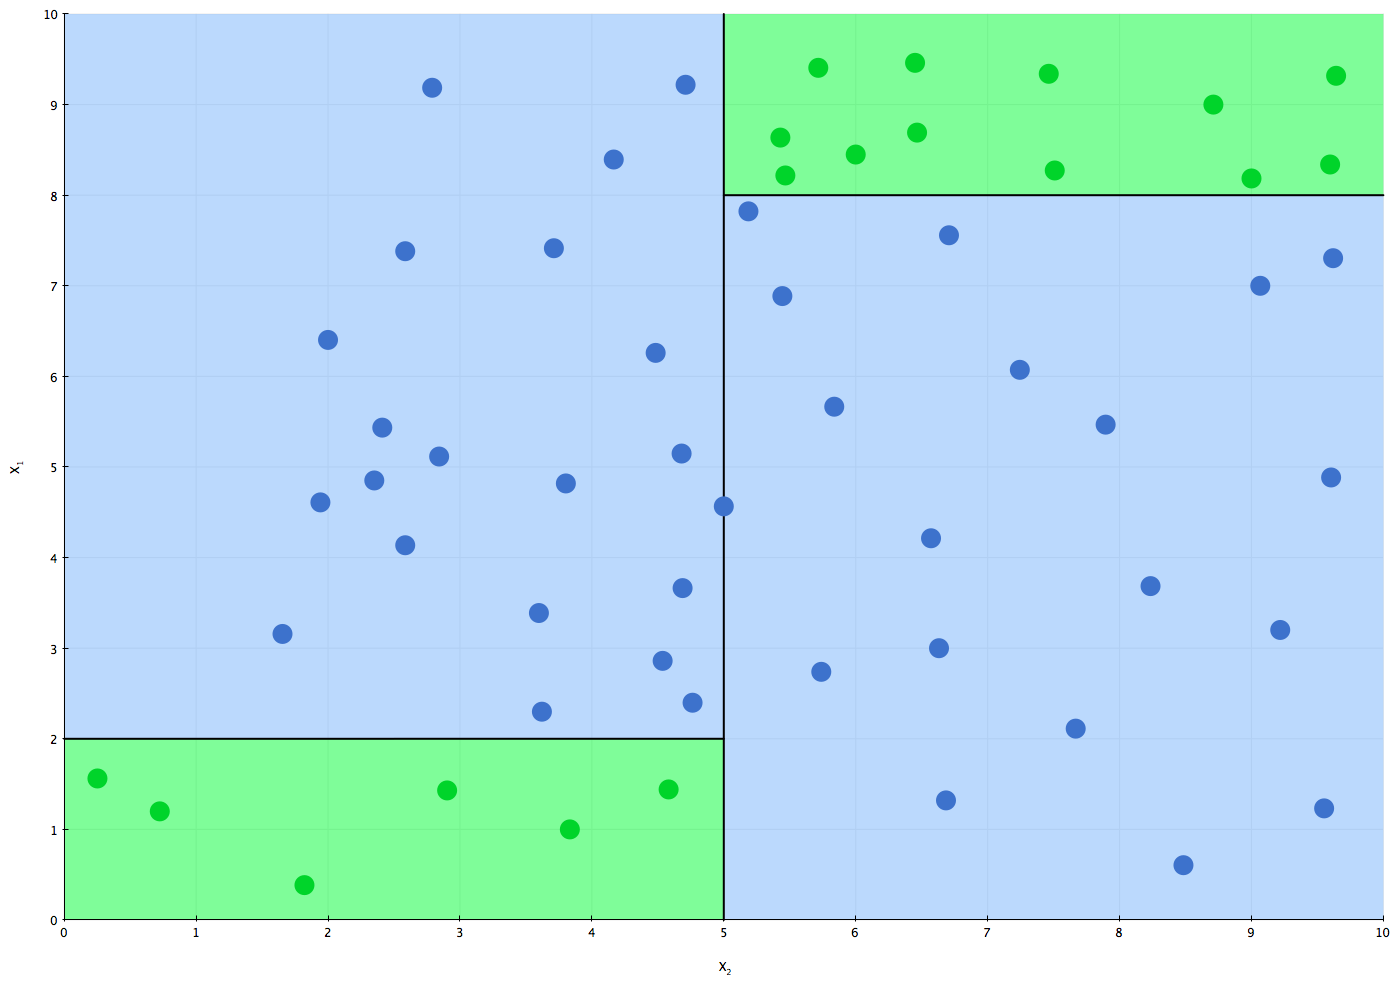
\includegraphics[width=0.5\textwidth]{images/preso_pic1_dec_trees_plot.png}}
      \hfill
      \subfloat[решающее дерево]{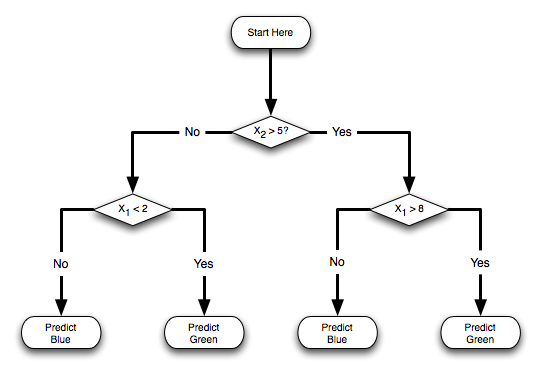
\includegraphics[width=0.5\textwidth]{images/preso_pic2_dec_trees.png}}
    \end{figure}

% оптимальное строить -- NP-полная задача, да еще и переобучение словим
% зато хорошо подходит для градиентного бустинга!

\vfill\vfill\vfill
{\tiny \color{gray} \url{https://alliance.seas.upenn.edu/~cis520/wiki/index.php?n=Lectures.DecisionTrees}}

\end{frame}


% гра-гра-гра-градиентный бустинг!!!
% строится итеративно, каждое следующее дерево исправляет ошибки предыдущего
% деревья простые и неглубокие -- эффективно применять

\begin{frame}\frametitle{Градиентный бустинг}
\begin{figure}[H]
    \center{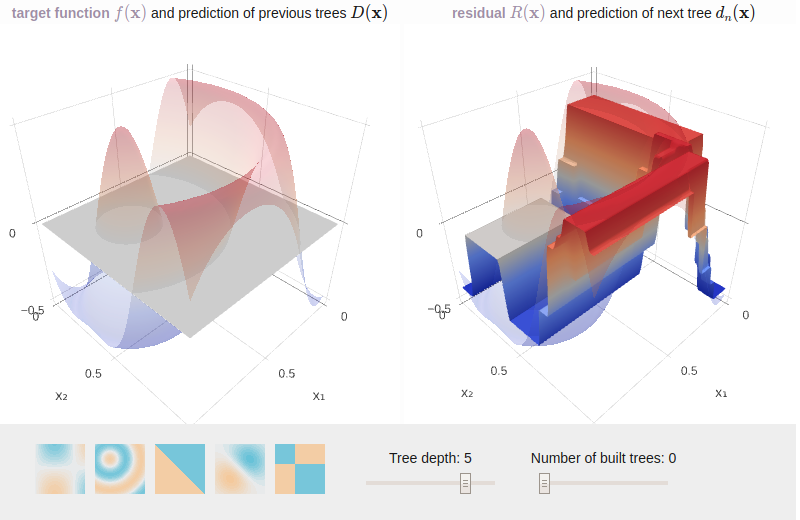
\includegraphics[width=0.9\linewidth]{images/preso_gb_0.png}}
\end{figure}
{\tiny \color{gray} \url{http://arogozhnikov.github.io/2016/06/24/gradient_boosting_explained.html}}
\end{frame}
\begin{frame}\frametitle{Градиентный бустинг}
\begin{figure}[H]
    \center{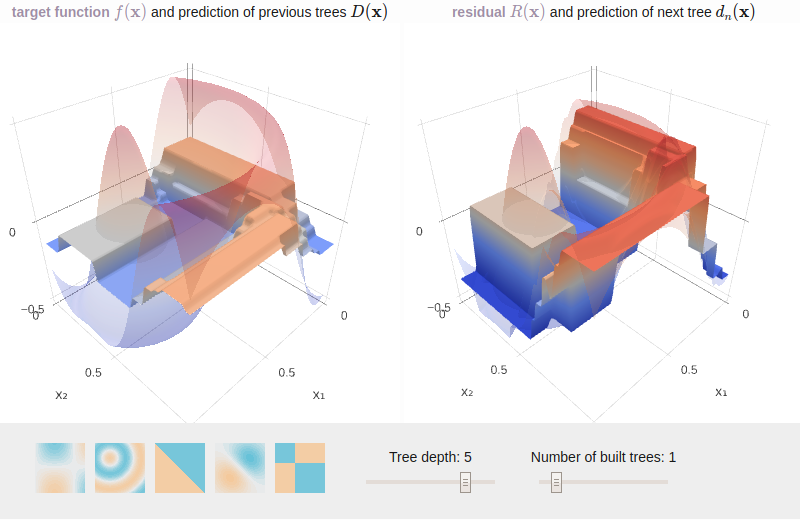
\includegraphics[width=0.9\linewidth]{images/preso_gb_1.png}}
\end{figure}
{\tiny \color{gray} \url{http://arogozhnikov.github.io/2016/06/24/gradient_boosting_explained.html}}
\end{frame}
\begin{frame}\frametitle{Градиентный бустинг}
\begin{figure}[H]
    \center{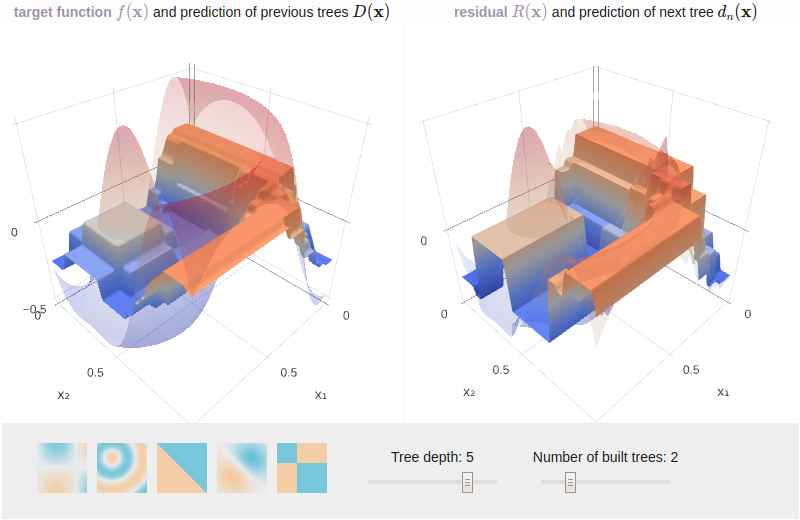
\includegraphics[width=0.9\linewidth]{images/preso_gb_2.png}}
\end{figure}
{\tiny \color{gray} \url{http://arogozhnikov.github.io/2016/06/24/gradient_boosting_explained.html}}
\end{frame}
\begin{frame}\frametitle{Градиентный бустинг}
\begin{figure}[H]
    \center{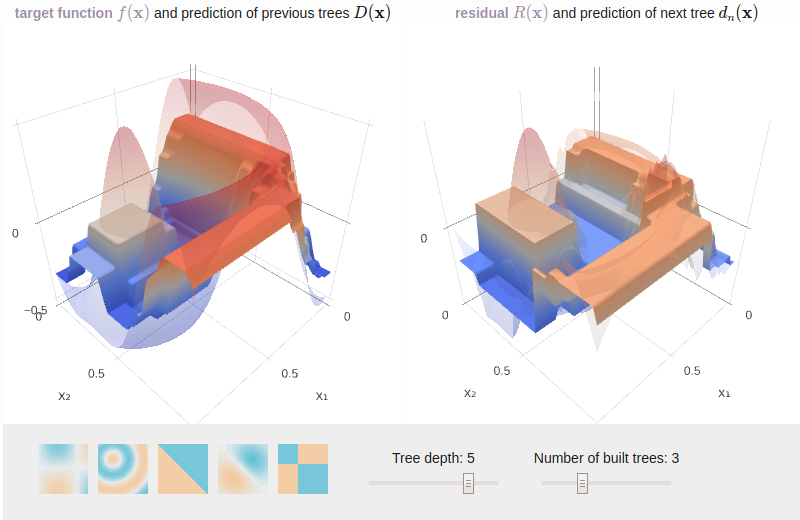
\includegraphics[width=0.9\linewidth]{images/preso_gb_3.png}}
\end{figure}
{\tiny \color{gray} \url{http://arogozhnikov.github.io/2016/06/24/gradient_boosting_explained.html}}
\end{frame}
\begin{frame}\frametitle{Градиентный бустинг}
\begin{figure}[H]
    \center{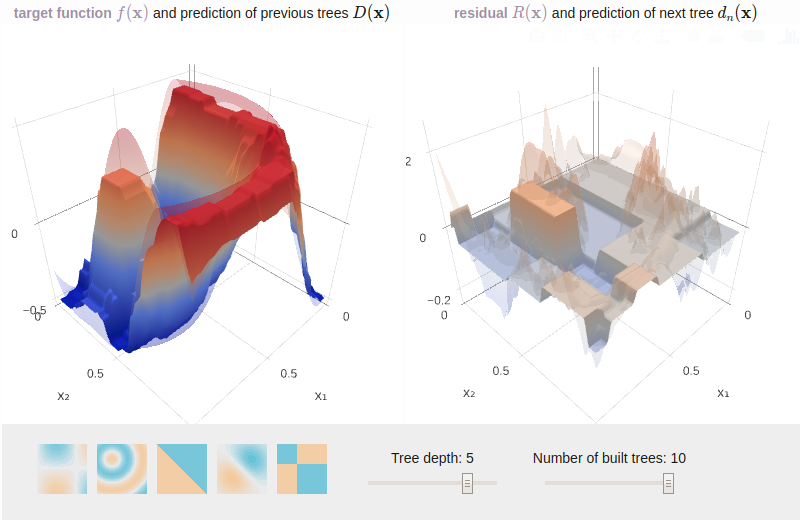
\includegraphics[width=0.9\linewidth]{images/preso_gb_10.png}}
\end{figure}
{\tiny \color{gray} \url{http://arogozhnikov.github.io/2016/06/24/gradient_boosting_explained.html}}
\end{frame}



\begin{frame}\frametitle{Эксперименты}
\begin{itemize}
    \item В момент $gentime$ прогнозируем погоду \\ в момент $time$
    \item $temperature\_delta = temperature - climate\_temperature$
    \item $X = \{x_i = (f^1_{i}, \cdots, f^M_i), i \in \overline{1..N}\}$, $y = \{y_i, i \in \overline{1..N}\}$
    \item $f_i$: прогнозы поставщиков, климатические данные, вспомогательные переменные
    \item Задача: добавить показания ближайших станций в момент $gentime$ (на 7 часов вперёд)
    \item Метрика: $RMSE(y, \hat{y}) = \sqrt{\frac{\sum^{n}_{i=1}{(y_i - \hat{y_i})^2}}{n}}$
    % задержки в получении данных?
\end{itemize}
\end{frame}


\begin{frame}\frametitle{Эксперименты: наивное решение}

Модели, обученные на всех краткосрочных горизонтах

\begin{figure}
\centering
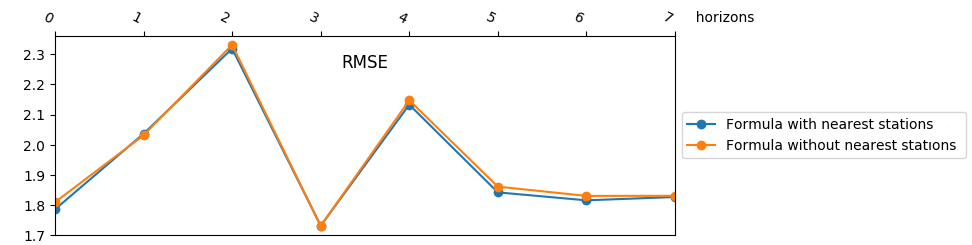
\includegraphics[width=\linewidth]{images/pic1_metrics_initial.png}
\end{figure}

% $fact1\_temperature\_delta$ на 151 месте из 250
\end{frame}



\begin{frame}\frametitle{Эксперименты: только первые N часов}

\begin{figure}\centering
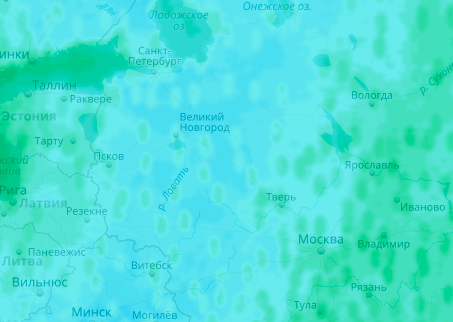
\includegraphics[width=\linewidth]{images/pic2_map.png}
\end{figure}
% $fact1\_temperature\_delta$ на 5 месте по эффекту, наравне с прогнозами температуры от поставщиков
\end{frame}



\begin{frame}\frametitle{Эксперименты: сглаживание}
\setlength\parindent{24pt}

\begingroup
\setlength\abovedisplayskip{0pt}

\begin{multline*}
smoothed\_fact\_temperature\_delta := \\\left\{
    \begin{array}{ll}
      fact \cdot (1 - \frac{dist}{max\_distance}) + forecast \cdot \frac{dist}{max\_distance},
      \\\indent \text{     if }dist \le max\_distance  \\
      forecast, \text{ if } dist > max\_distance
    \end{array}
  \right.,
\end{multline*}
\endgroup

{\scriptsize 
    \indent где $fact$ -- исходное значение с одной из ближайших станций, \\
    \indent $dist$ -- расстояние до неё, $forecast$ -- прогноз поставщика
}

\begin{figure}
\centering
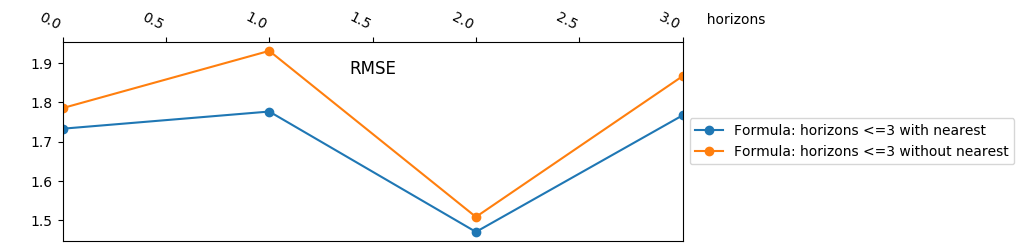
\includegraphics[width=\linewidth]{images/pic3_metrics_final.png}
\end{figure}

% Сглаженные температуры с двух ближайших станций оказались на 1 и 4 местах по влиянию на ответ модели.
% пятен нет
% это пару дней как в проде!
\end{frame}


\begin{frame}\frametitle{Дальнейшее развитие}

\begin{itemize}
    \item не только $temperature\_delta$
    \item кросс-валидация
    \item параметры градиентного бустинга
    \item другие способы сглаживания
\end{itemize}

\begin{figure}
\centering
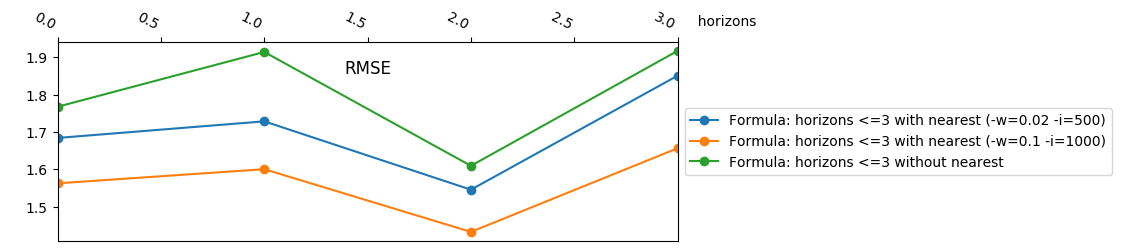
\includegraphics[width=\linewidth]{images/pic4_params.png}
\end{figure}

\end{frame}



\end{document}